\documentclass{beamer}
\mode<presentation>
{
 \usetheme{Frankfurt}
 \setbeamercovered{transparent}
}
\usepackage[russian]{babel}
\usepackage[utf8]{inputenc}

\usepackage{mathptmx}
\usepackage{graphics}
\usepackage[scaled=.90]{helvet}
\usepackage{courier}
\usepackage[T1]{fontenc}

\usepackage{listings}
\lstset{language=Python, numberstyle=\tiny, keywordstyle=\color{blue},numbers=left,commentstyle=\color{green},
basicstyle=\footnotesize}

\title{ Использование файловых систем в качестве абстракции для доступа к
системам управления мобильных роботов и мехатронных устройств}

\author{К.Б. Кирсанов, Е.А. Прысев}
%\institute[sensorika]
%{ИПМ им. Келдыша РАН}

\date{27.06.2013 // Объединённый семинар по робототехническим системам}

\beamerdefaultoverlayspecification{<+->}

\begin{document}

\begin{frame}
\titlepage
\end{frame}

\begin{frame}
\frametitle{Содержание}
\tableofcontents
\end{frame}


\section{Введение}
\begin{frame}
\frametitle{Введение}
\framesubtitle{Формулировка целей исследования}

Необходимо обеспечить управление отдельными мехатронными устройствами и
различными роботами в рамках пространственно-распределенной гетерогенной сети.
\begin{itemize}
  \item<1>\emph{пространственно-распределенной} -  подсети в ИПМ, РГГУ, Станкин,
	ДВФУ (Владивосток)
  \item<1>\emph{гетерогенность} -  роботы АМУР разных поколений,
  Robotino(Festo) 2 вида, Kuka, оборудование AXIS, Smartec
\end{itemize}

Требуется создать единообразный интерфейс управления.
\end{frame}

\begin{frame}
\frametitle{Введение}
\framesubtitle{Задачи}
\begin{itemize}
 	\item<1>Как сформировать управляющую команду для конкретного
 	мехатронного устройства
 	\item<1>Как её доставить, учитывая распределённость
 	сети, права доступа и т.п.
\end{itemize}
\end{frame}

\section{Файловая система как интерфейс}
\begin{frame}
\frametitle{Введение}
\framesubtitle{Способы управления и программирования}
Абсолютное большинство современного ПО мобильных роботов и мехатронных систем
используют следующие способы программирования и управления:
\begin{itemize}
 	\item<1> Библиотеки для языков общего назначения
	\item<1> Фреймворки для языков общего назначения
	\item<1> Веб-интерфейсы
	\item<1> Собственное ПО с графическим интерфейсом
	\item<1> Фреймворки DSL
\end{itemize}

\end{frame}

\begin{frame}
\frametitle{Интерфейсы}
\framesubtitle{Интерфейсы в программировании}

\em{Интерфейс} — совокупность возможностей взаимодействия двух систем,
устройств или программ, определённая их характеристиками, характеристиками соединения, сигналов обмена и т. п.
(wikipedia)
\\

Для обеспечения взаимодействия с мехатронными устройствами требуется
создание интерфейсов, как пользовательских (для человека), так и программных (API).

Не существует единого общепризнанного стандарта на интерфейсы систем
управления роботами и мехатронными устройствами.
\end{frame}


\subsection{GUI}
\begin{frame}
\frametitle{GUI}
\framesubtitle{Graphical User Interface}
Графический интерфейс пользователя благодаря своей наглядности позволяет быстро приступить к работе
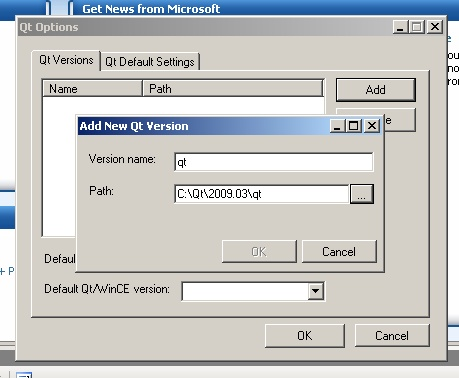
\includegraphics[width=8cm]{button.jpg}
\end{frame}

\begin{frame}
\frametitle{GUI}
Но не всегда\ldots
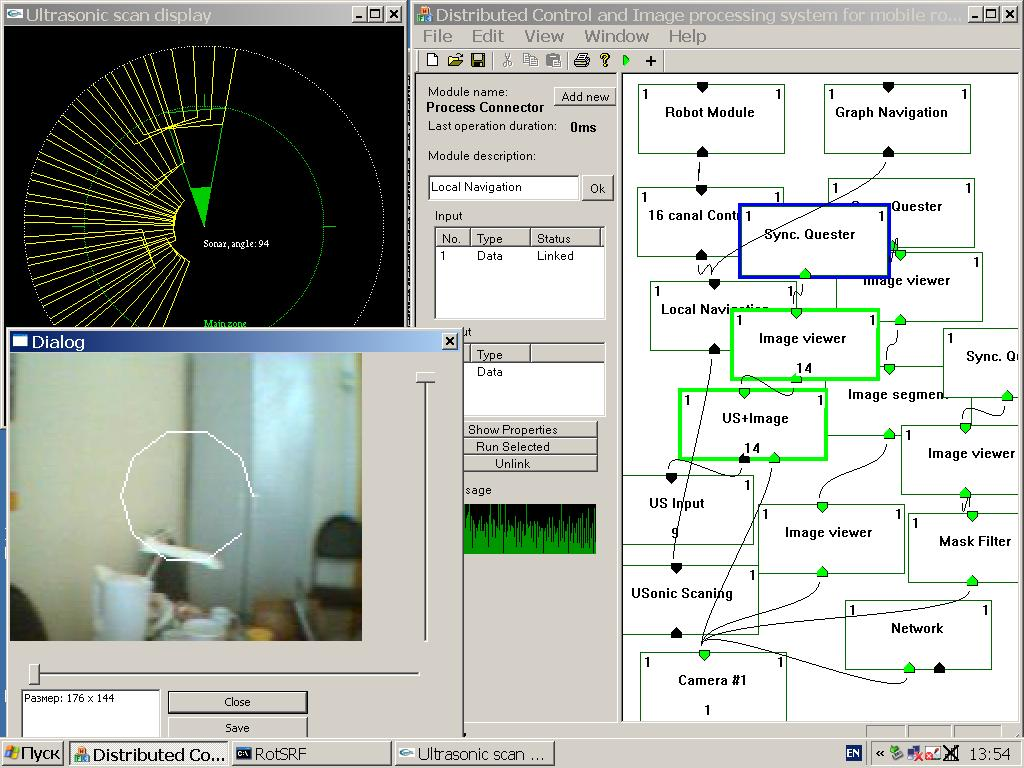
\includegraphics[width=7cm]{hell.jpg}
\end{frame}

\subsection{API}
\begin{frame}
\frametitle{API}
\framesubtitle{Application Programing
Interface - Интерфейс программирования приложений}
Интерфейс программирования приложений — набор  классов, процедур, функций, структур и 
констант, предоставляемых приложением (библиотекой, сервисом) для использования 
во внешних программных продуктах. 
\lstinputlisting{code.py}
\end{frame}

\begin{frame}
\frametitle{API}
\framesubtitle{Достоинства и недостатки, по сравнению с GUI}
\begin{itemize}
  \item<1> API более гибкий
  \item<2> Выше порог вхождения
  \item<2> Требуются специфичные знания, связанные с конкретными языками,
  платформами и алгоритмами
\end{itemize}

Интерфейсы управления мехатронными устройствами могут быть весьма разнообразны,
причем для программиста, разрабатывающего ПО, программный интерфейс 
(API) фактически становится пользовательским, 
так как для него язык программирования и программа на этом языке становится
инструментом, аналогичным мышке, в руках “обычного” пользователя.
\end{frame}


\begin{frame}
Файловая система оказывается довольно удачной абстракцией для доступа к данным и
состояниям системы управления:
\begin{itemize}
  \item<1> Работа с ней требует общеизвестных навыков работы с файлами и не
  нуждается в дополнительном изучении
  \item<1> Она проста в реализации, что позволяет быстро вводить новые
  мехатронные устройства в работу.
 
\end{itemize}
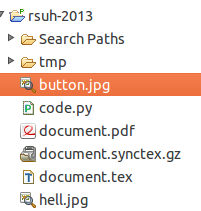
\includegraphics[width=2.3cm]{file.png}
\end{frame}

\subsection{FUSE}
\begin{frame}
\frametitle{Plan 9}
Операционная система Plan 9 (Bell Labs - 1980) -
http://www.plan9.bell-labs.com/

\begin{itemize}
  \item<1> Все ресурсы представлены как файлы и доступны в иерархической
  файловой системе
  \item<1> Локальные и удалённые ресурсы не различаются
  \item<1> Каждая группа процессов имеет собственное пространство имён,
  которое собирается из файловых иерархий, предоставленных
  различными ресурсами
\end{itemize}
\end{frame}

\begin{frame}
\frametitle{Plan 9 - фильм и ОС}
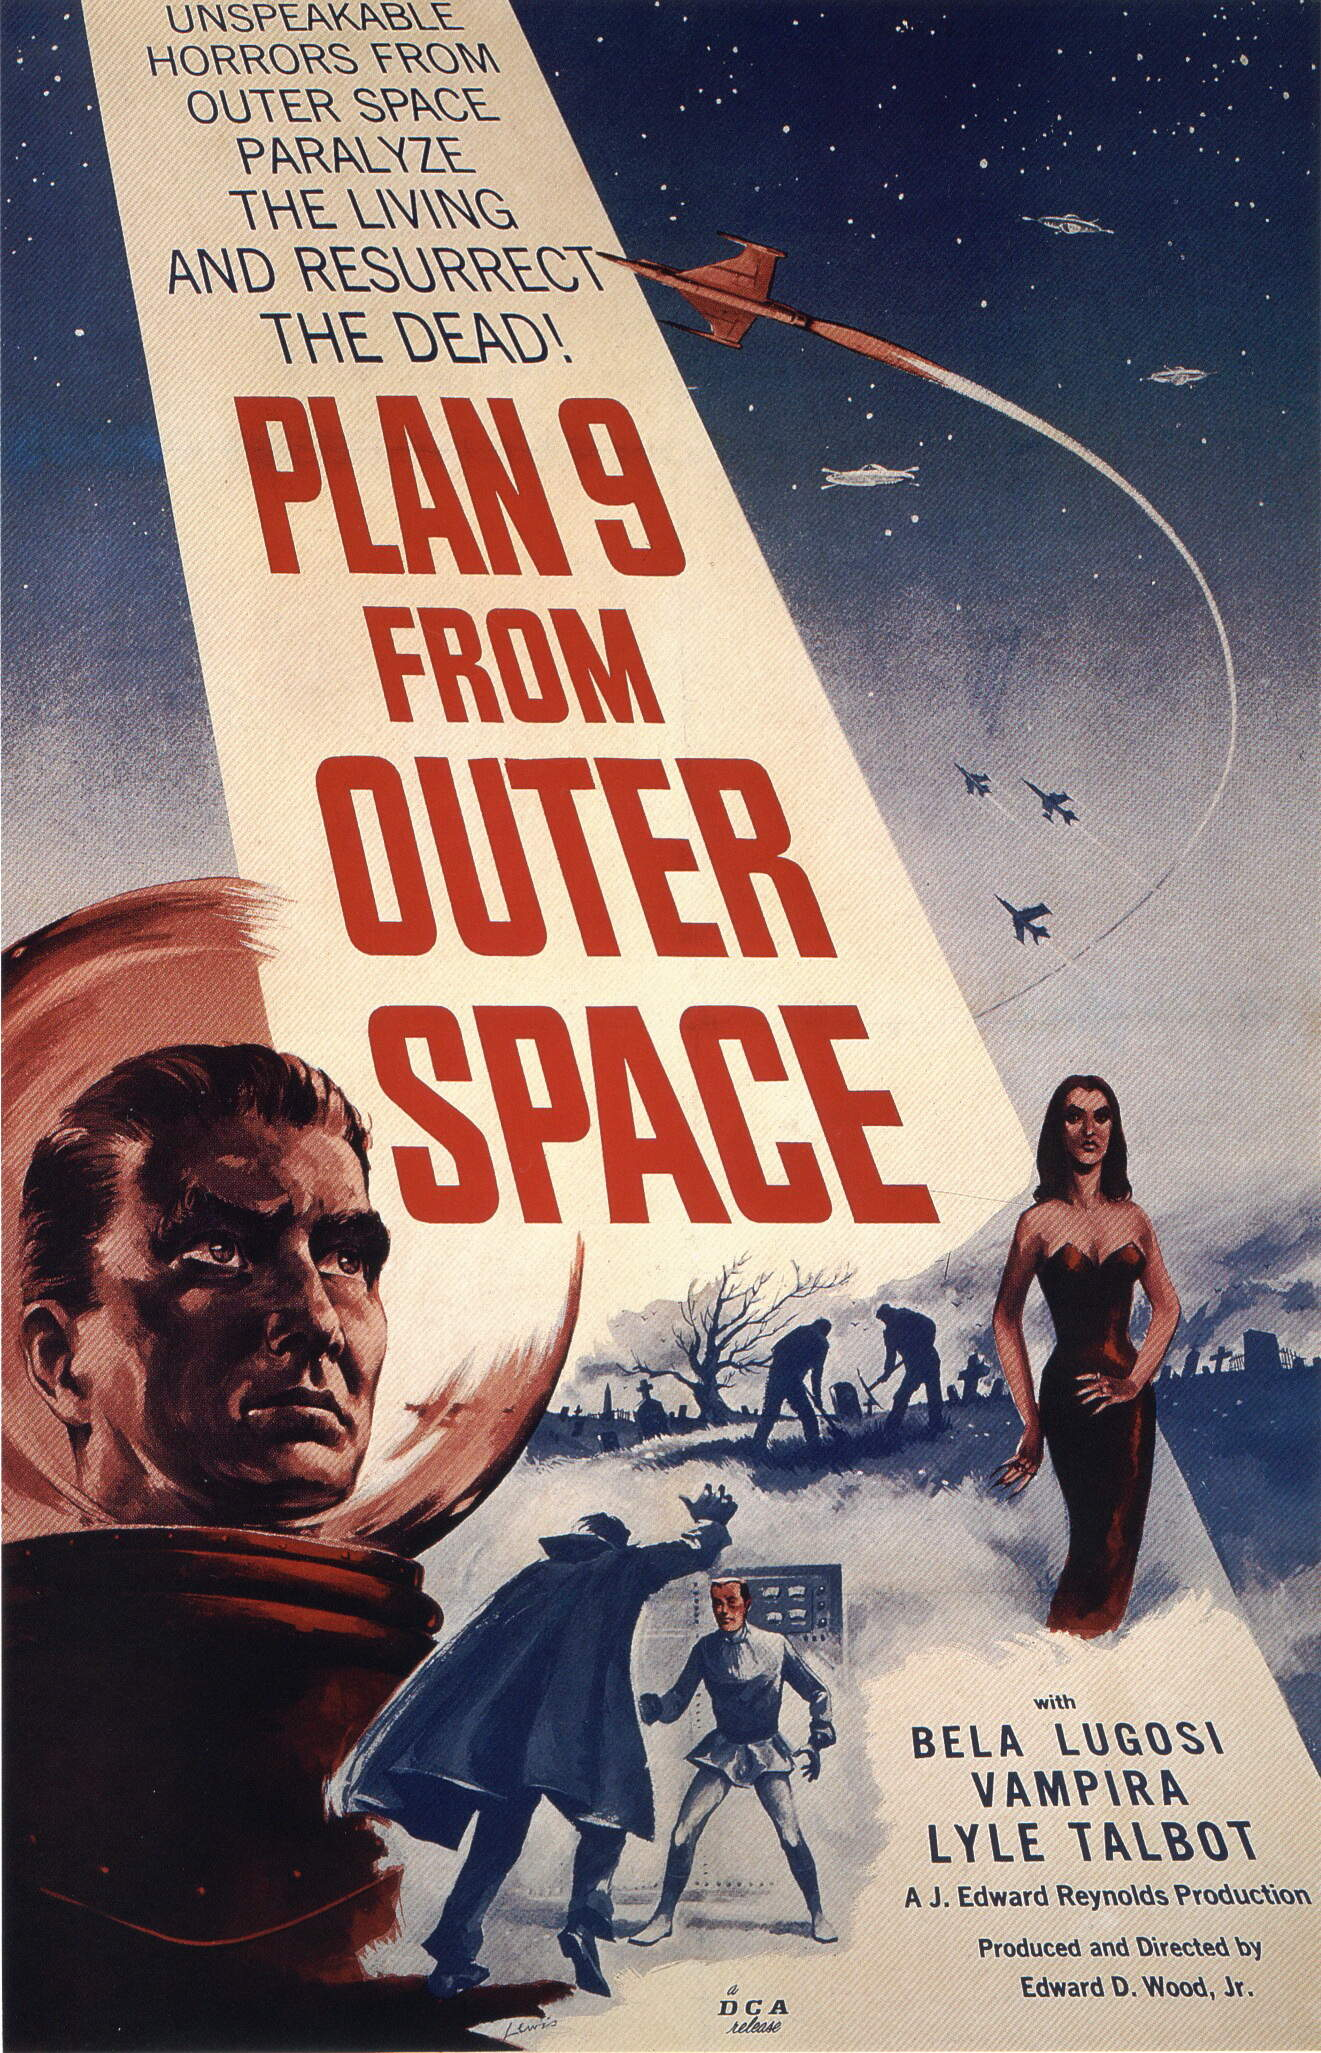
\includegraphics[width=4.5cm]{plan9_film.jpg}

\includegraphics[width=5.3cm]{plan9_os.jpg}

\end{frame}

\begin{frame}
\frametitle{FUSE - Filesystem in Userspace}
Для реализации такого рода файловой системы (ФС) необходимо либо написать
собственный драйвер ФС, исполняемый на уроне ядра, или же воспользоваться
ФС уровня пользователя FUSE.

FUSE это модуль для ядер UNIX-подобных операционных систем, обеспечивающий весь
функционал работы с ФС без необходимости предоставления привилегий администратора и внедрения кода в ядро.

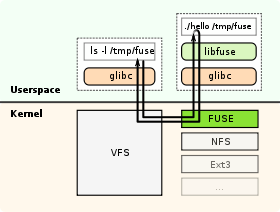
\includegraphics[width=4.3cm]{fuse.png}
\end{frame}

\subsection{Чтение}
\begin{frame}
\frametitle{Чтение}
\begin{itemize}
\item<1> Например, изображение с видеокамеры будет отображаться на файлы
cam1.bmp и cam1.jpg в форматах bitmap и jpeg соответственно, что позволит
проверить работу видеокамер, получить изображение и выполнить другие простейшие
операции встроенным в ОС ПО, не прибегая к программированию или стороннему ПО.
\item<1> Для обеспечения управления, которое реализуется через запись в файл,
такое простое отображение оказывается уже недосточным. С одной стороны
возникают коллизии совместного доступа, а с другой - тривиальных данных оказывается явно не
доcтаточно для управления (а только такие и можно ввести в стандартном текстовом
редакторе).
\end{itemize}
\end{frame}

\subsection{Управление}
\begin{frame}
\frametitle{Управление - пример}
Пусть текущее значение управления ШИМ отображается на файл ./pwm.cmd в виде
текста ``255``, что соответствует максимальному сигналу управления. Чтобы
отключить ШИМ, достаточно открыть данный файл в любом текстовом редакторе,
добавить новую строку и записать в нее ``0``.
Таким образом файл примет вид:
\lstinputlisting{code2.py}
Первая строчка обозначает текущее значение ШИМ, а вторая - каким значением его
следует заменить. В момент сохранения файла специальное ПО модифицирует
программу управления так, чтобы на ШИМ поступал ``0``. 
При следующем открытии файла в нем будут те же строки, что позволит корректно его 
модифицировать в дальнейшем.
\end{frame}

\subsection{Программирование}
\begin{frame}
\frametitle{Программирование}
Но замена константой не всегда оказывается достаточной. По этой причине была
реализована возможность написания простых программ в том же файле.
\lstinputlisting{code3.py}
Переменной x на каждом витке цикла управления автоматически присваивается
значение параметра и, по завершении программы, это значение и подается на
управление.
\end{frame}


\subsection{Протоколирование}
\begin{frame}
\frametitle{Протоколирование}
Отдельно следует упомянуть задачу протоколирования. История (шлейф) состояний
отображается на соответствующие файлы с расширением .history. Файл, в котором
отображается история показаний ультразвукового датчика (УЗ), имеет
следующий вид:
\lstinputlisting{code4.py}
Где первый столбец - время измерения относительно старта системы в секундах, а
второй - данные измерений.
\end{frame}

\begin{frame}
\framesubtitle{Сравнение файловой системы и ООП API}
Пример решения задачи ``напечатать на экране данные УЗ датчика'':
ООП API
\lstinputlisting{fs-samiple1.py}
Файловая система
\lstinputlisting{fs-samiple2.py}
\end{frame}

\section{Сетевое взаимодействие}
\subsection{TCP/IP}
\begin{frame}
\frametitle{Пример Robotino}
Практически всё ПО для мобильных роботов в качестве основного протокола
использует TCP/IP. Это семейство протоколов стало стандартом де-факто.

Для адресации используется IP адрс: 32-битовое число. Удобной формой записи
является запись в виде четырёх десятичных чисел значением от 0 до 255,
разделённых точками.
\lstinputlisting{robotino.cpp}
\end{frame}

\subsection{Служба Каталогов}
\begin{frame}
\frametitle{Служба Каталогов}
\begin{itemize}  
\item<1>Чтобы через протокол TCP/IP обратиться к конкретному роботу или
мехатронному устройству, нужно знать IP-адрес
\item<1>Требуется создание службы катлогов, а также классификатора роботов и
мехатронных устройств, которые позволят получать доступ без знания IP-адреса
\item<1>Пример такой службы - DNS (Domain Name System — система доменных имён)
в сети интернет. DNS ставит в соответствие имени домена - IP-адрес
\end{itemize}
\end{frame}

\subsection{DNS}
\begin{frame}
\frametitle{Свойства DNS}
\begin{itemize}
\item<1>Распределённость администрирования. Ответственность за разные части
иерархической структуры несут разные люди или организации.
\item<1>Распределённость хранения информации. Каждый узел сети в обязательном
порядке должен хранить только те данные, которые входят в его зону ответственности и (возможно) адреса 
корневых DNS-серверов.
\item<1>Кеширование информации. Узел может хранить некоторое количество данных
не из своей зоны ответственности для уменьшения нагрузки на сеть.
\end{itemize}
\end{frame}

\begin{frame}
\frametitle{Свойства DNS}
\framesubtitle{Продолжение}
\begin{itemize}
\item<1>Иерархическая структура, в которой все узлы объединены в дерево, и
каждый узел может или самостоятельно определять работу нижестоящих узлов, или делегировать (передавать) 
их другим узлам.
\item<1>Резервирование. За хранение и обслуживание своих узлов (зон) отвечают
(обычно) несколько серверов, разделённых как физически, так и логически, что
обеспечивает сохранность данных и продолжение работы даже в случае сбоя одного из узлов.
\end{itemize}
\end{frame}

\subsection{DNS для роботов}
\begin{frame}
\frametitle{DNS для роботов}
Специфика ``Сети роботов`` не позволят напрямую использовать DNS
\begin{itemize}
  \item<1> Переход роботов из одной сети в другую 
  \item<1> Нестабильность сети
  \item<1> Необходимость сохранения работоспособности при отключении от сети
\end{itemize}
\end{frame}

\begin{frame}
\frametitle{Единый каталог ресурсов - LDAP}
%При построении  робототехнической лаборатории с многопользовательским доступом 
%можно выделить следующие основные проблемы:
%\begin{itemize}
%\item<1> Cопряжение устройств различных производителей (как активных, например,
%роботов, так и пассивных - например, видеокамера наблюдения) и их объединение в
%единое пространство
%\item<1> Разграничение доступа к ресурсам лаборатории. Гарантия предоставления
%выделенного оборудования в заявленное время. Гарантия монопольного
%использования
%\item<1> Требования к квалификации обслуживающего персонала лаборатории
%\end{itemize}
\end{frame}

\begin{frame}
\frametitle{DNS/LDAP для роботов}
\framesubtitle{Наше решение}
Разработано аналогичное DNS ПО, со следующим алгоритмом:
\begin{itemize}
  \item<1>Копия ПО службы каталогов включается в соств любого ПО,
  устанавливаемого на бортовую ЭВМ
  \item<1>При запуске проверяется наличие сервера имён на локальном IP
  \item<1>Если он не находится, то поиск расширяется на локальную сеть
  \item<1>Если он не находится, то запускается ПО службы каталогов
\end{itemize}
\end{frame}

\subsection{Классификация мехатронных устройств}
\begin{frame}
\frametitle{Классификация мехатронных устройств}
Для доступа к устройствам их необходимо классифицировать.
Классификация, как правило, ведется по:
\begin{itemize}
  \item<1> Месту - в каком роботе находится мехатронное устройство. Характерно
  для ООП. Строится естественным образом
  \item<1> Типу (данных) управления - с какими устройствами может
  взаимодействовать данное. Характерно для средств графического
  программирования
\end{itemize}
\end{frame}

\begin{frame}
\frametitle{Пример использования классификаций}
\framesubtitle{ООП API Lego}
\lstinputlisting{lego.cpp}
\end{frame}

\begin{frame}
\frametitle{Пример использования классификаций}
\framesubtitle{Визуальное программирование в Robotics Studio}
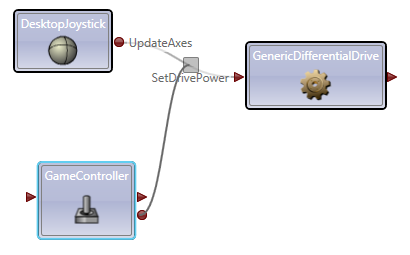
\includegraphics[width=8cm]{rs.png}
\end{frame}

\begin{frame}
\frametitle{Текущее состояние работ}
Готово:
\begin{itemize}
  \item<1> Файловая система как интерфейс доступа
  \item<1> Сетевая инфраструктура канального уровня (провода, IP сеть, VPN
  туннели)
  \item<1> Прототипы интерфейсов
  \item<1> Программы-трансляторы для оборудования Axis, Smartek
\end{itemize}
Осталось незавершённым:
\begin{itemize}
  \item<1> Классификации
  \item<1> Служба каталогов и разграничения доступа
  \item<1> Программы-трансляторы для оборудования Festo и ABB
\end{itemize}
\end{frame}
\end{document}